\section{Forwarding in opportunistic networks}
\label{forwarding}

Opportunistic networks are highly dynamical network, connections are not durable like internet ones and contact network can be characterized by more than one connected components dynamics, even without a giant connected component at all. For this reason forwarding decision might be not so oblivious and using traditional forwarding schemes might lead to limitations in terms of both efficiency and effectiveness. \\ In this section we describe several algorithms that could be used for forwarding a message in a dynamic, Delay Tolerant Network (DTN), with particular regards to algorithms that exploit network topology informations.

\subsection{Non social-based algorithms}
\label{f_non_social}
Before talking about social-based algorithm we want perform a non exhaustive survey of canonical forwarding algorithm, that ones which does not exploit any network topology information. This kind of algorithms are a fundamental reference framework even during analysis of newer forwarding algorithms because they can provide a solid base for benchmarking. We can individuate three canonical forwarding algorithm:

\begin{description}
\item[Wait] consists in merely holding the message until recipient is directed encountered. Pretty ineffective, but it provide a lower bound in term of both delivery cost and delivery ratio.
\item[Flood] used also in several routing protocols (eg.OSPF) for network image construction, consists in a flooding through the entire system. Represent the upper bound in term of both delivery cost and delivery ratio.
\item[MCP] \emph{Multiple-Copy-multiple-hoP}, it's a mix of the previous approach. Each node can forward only a predefined number of copies for each message; each message has also a TTL measured in Hops (like common IP packets). It represent a pretty efficient and effective forwarding scheme for naive algorithms.\end{description} 

\subsection{Social-based algorithms}
\label{f_social}
Basic approaches introduced previously does not make any assumption on contact network so a newer set of forwarding algorithm have been investigated in the last decade.\\ Considering that humans will carry these mobile nodes enable us to make new assumptions that could be exploited in forwarding decisions, so we will perform a qualitative survey on forwarding algorithms which exploit this consideration in order to extract concepts and measures behind forwarding decision-making:

\subsubsection{Label algorithms}
This approach exploit the human dimension of the problem, in fact messages are forwarded only to encountered nodes with the same (or also similar) interest of the recipient. The concept of similarity of interest is important because typically similar tends to stay close, in other words this forwarding algorithm exploit communities structures (eg. \emph{k-cliques}) which are characteristic of small-world networks.

\subsubsection{Rank algorithms} 
Here the focus is on node centrality, this is the key measure considered in forwarding decisions. For example in \emph{Greedy Rank Algorithm} messages are forwarded only to neighbours that have higher centrality value, or also can be performed sort of climb for reaching nodes with maximum rank, and then a descent to the recipient\cite{PhysRevE.64.046135}, but identifying the maximum rank value in a distributed system is not cost-free and in general assuming the knowledge of the whole network structure or global values could be unrealistic, so this kind of algorithms typically use heuristics to estimate centrality values.

\subsubsection{Bubble algorithms}
\label{f_bubble}
Bubble algorithm\cite{bubble} family basically play with both rank and labels in order to enhance efficiency in terms of minimizing in flight copies. The approach is pretty interesting due to it considers two level of ranking: a \emph{global ranking} which coincide with measure of centrality w.r.t. the whole network, and a \emph{local ranking} that consider centrality w.r.t. nodes in the same community. Successively it mixes these notions of rank with the community membership.\\
The following algorithm's sketch\ref{r_bubble_alg} shows how these elements are combined.

\begin{algorithm}
\caption{Bubble RAP forwarding algorithm}
\label{r_bubble_alg}
\begin{algorithmic}
\FOR{$neighbor$ such that $neighbor \in neighborhood(node)$  } 
\IF{$LabelOf(node) == LabelOf(recipient)$} 
	 \IF{$LabelOf(neighbor) == LabelOf(recipient)$ \AND $LocalRank(neighbor ) > LocalRank(node)$} 
			\STATE{$forwardMessageTo(neighbor)$}
 		\ENDIF 
 \ELSE
 	 \IF{$LabelOf(neighbor) == LabelOf(recipient)$ \OR $GlobalRank(neighbor) > GlobalRank(node)$} 
 	 \STATE{ $forwardMessageTo(neighbor)$}
 		\ENDIF 
 \ENDIF
 \ENDFOR
\end{algorithmic}
\end{algorithm}

In \cite{bubble} experimental results have shown that this forwarding strategy is effective like MCP (slightly less than flooding algorithm) but with a notable difference in term of delivery cost. In figure\ref{fig:bubblerap-performance} are reported the result of an experiment with two main communities.

\begin{figure}[h!]
	\begin{center}
    \label{fig:bubblerap-performance}
    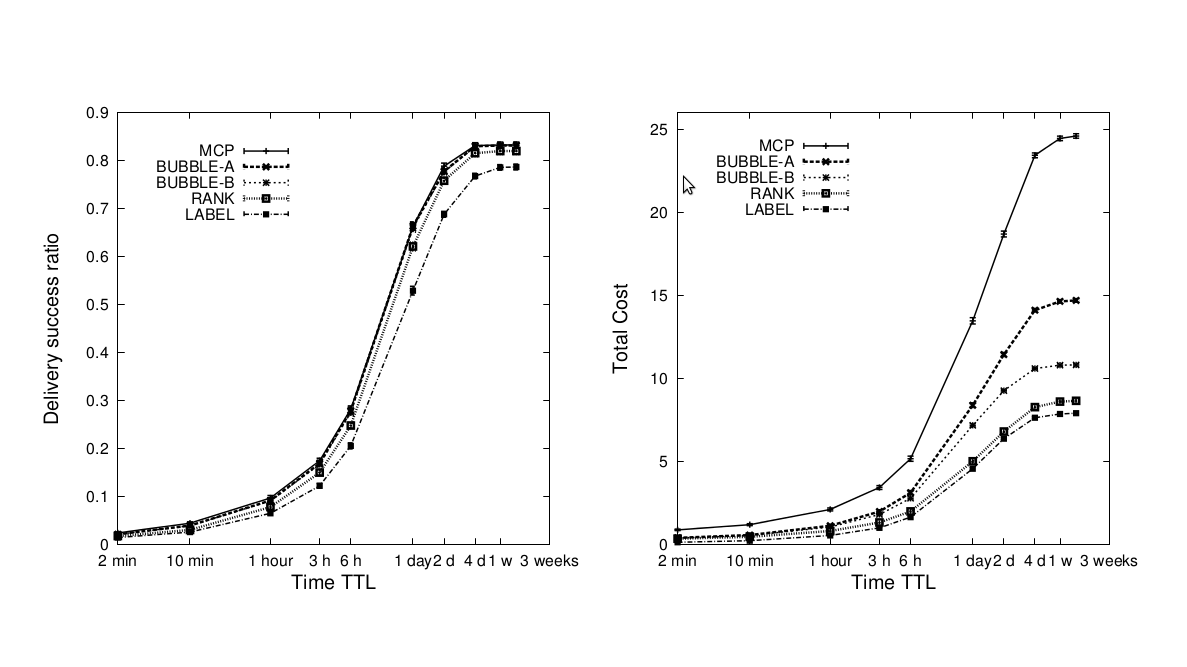
\includegraphics[scale=0.35]{img/bubblerap-performance.png}
    \caption{Comparison of several algorithms in two-community experiment based on \emph{Haggle Project} data sets performed in\cite{bubble}}
  \end{center}
\end{figure}
